\chapter{Fortran Projects}


\vspace{0.5cm} 

    \FloatBarrier
    \section{Installing Fortran Compiler} \label{sec:FortranIns}
    
As it has been said before, we need now the compiler of the programming language we are interested in. Hence, Intel\textregistered\hspace{0.05cm} Fortran Compiler must be installed in the computer and it should be recognized by the Visual Studio environment (previously installed). We are going to use an academic license, follow the steps below:
%We need now the Fortran Compiler developed by Intel, it is in charge of generating code for IA-32 and %Intel 64 processors (and some other compatible processors) and have to be installed through Intel %Parallel Studio XE.

%\vspace{1cm}

\begin{IN}
    \begin{itemize}
        \item Please notice that Visual Studio \textbf{MUST be installed in the first place}. Do not continue with this installation if the IDE is not already installed in your computer.
        \item The packages used for the installation of Intel\textregistered\hspace{0.05cm} Fortran Compiler are the \textit{Intel\hspace{0.04cm}\textregistered\hspace{0.05cm} oneAPI Base Toolkit} and \textit{Intel\hspace{0.04cm}\textregistered\hspace{0.05cm} oneAPI HPC Toolkit}. Try to install always the latest version of the compiler offered by Intel in order to ensure the compatibility with the latest version of Visual Studio.
    \end{itemize}
\end{IN} 

\newpage
\begin{itemize}
    \item[a)] Downloading \textit{Intel\hspace{0.04cm}\textregistered\hspace{0.05cm} oneAPI Base Toolkit} for students:
    \begin{enumerate}
        \item We first go to the official website of Intel Developer Zone, click on the next url to see the available tools:
   
        \url{https://software.intel.com/content/www/us/en/develop/}
        
        \url{articles/free-intel-software-developer-tools.html}
        
        \item First of all, sign in if you already have an Intel account, you can find the option in the right upper part of the window. If you do not have an Intel Account create it by clicking on \textit{Sign In} and then \textit{Sign up here}.
            \begin{itemize}
                \item Fill in all the Personal Information (you can use your institutional email in the field \textit{Business Email Address}). Click on \textit{Next Step} when finished.
                \item Click on \textit{Submit} for the Terms and Conditions.
                \item Verify your e-mail address by clicking on the link available in the verification email you have received.
                \item Sign In now with your new account in the previous url. 
            \end{itemize}
        \item In order to obtain first the Base Toolkit click on \textit{Get the Base Kit} (Figure \ref{fig:Proceso2A}).
        \item Now choose from the available options, in this case \textit{Windows/Web \& Local/Local} and click on \textit{Download} (Figure \ref{fig:Proceso2B}).
        \item Save the file in your computer.
    \end{enumerate}   
    
    \item[b)] Downloading \textit{Intel\hspace{0.04cm}\textregistered\hspace{0.05cm} HPC Toolkit} (High-Performance Computing) for students:   
    \begin{enumerate}
        \item Follow the same process in order to download the HPC Toolkit clicking now on \textit{Get the HPC Kit} in the third step (Figure \ref{fig:Proceso2A}).
        \item Save the file in your computer.
    \end{enumerate} 

    \item[c)] Installing both tools:
    \begin{enumerate}
        \item Now you have both installers downloaded in your computer. Double click first on the installer of the Base Toolkit, named something similar to:
        
         \texttt{w\_BaseKit\_p\_XXXX.X.X.XXXX\_offline.exe}.
        \item Accept the installation as an administrator and click on \textit{Extract} the temporary files needed by the installer. Wait until the process finishes. 
        \item In the first window that appears click on \textit{Continue} and in the next one mark the option \textit{I accept the terms of the license agreement}, click on \textit{Continue} for the Recommended Installation (Figure \ref{fig:Proceso2C}). 
        \item Now the installer shows warnings related to the needed modules (this step should not block the installation so we continue with the process), click on the right arrow. 
        \item Make sure the integration with your current version of Visual Studio is marked (Figure \ref{fig:Proceso2D}), click on the right arrow.
        \item In the last window you have to decide about consenting or not the collection of private information, choose your options and click on \textit{Install}.
        \item Wait until the process finishes (it can be slow) (Figure \ref{fig:Proceso2E}). 
        \item When finished click on \textit{Go to Installed Products} and then close the installer. 
        \item Follow the same process described with the other installer, named something similar to \texttt{w\_HPCKit\_p\_2021.1.0.2682\_offline.exe}.
    \end{enumerate}
\end{itemize}

After the installation has finished we can start creating our Fortran projects and executing programs.

\begin{figure}
    \centering
    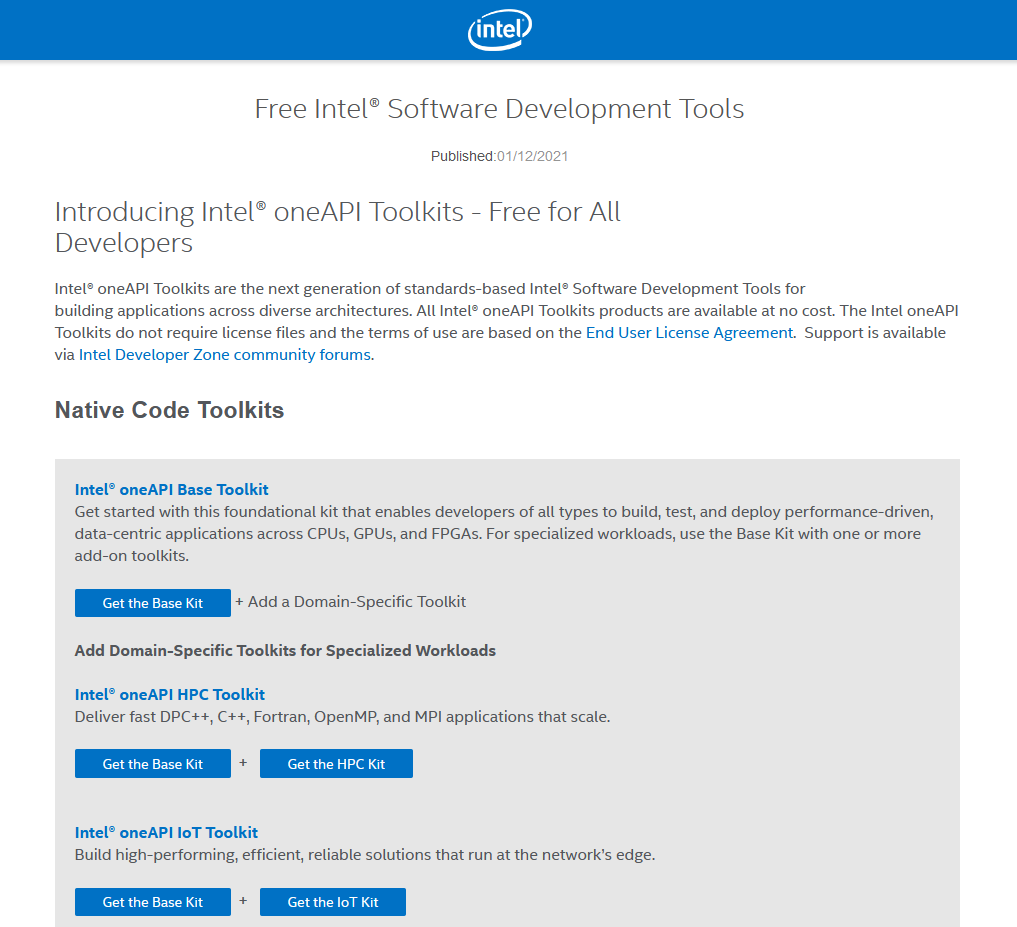
\includegraphics[width=\textwidth]{Figures/Proceso2A}
    \caption{This website shows different toolkits offered by Intel. We are interested in the Base toolkit (always needed) and HPC toolkit (High-Performance Computing).}
    \label{fig:Proceso2A}
\end{figure}

\begin{figure}
    \centering
    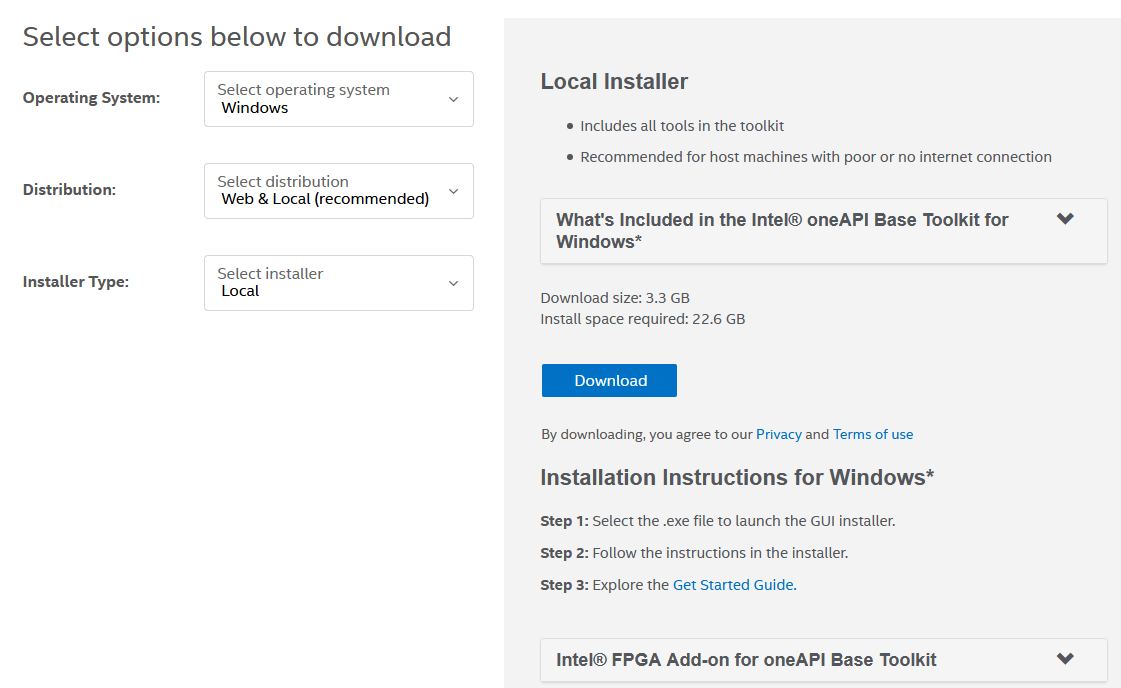
\includegraphics[width=  \textwidth]{Figures/Proceso2B}
    \caption{Second step of the download, select these options and click on \textit{Download}.}
    \label{fig:Proceso2B}
\end{figure}

\begin{figure}
    \centering
    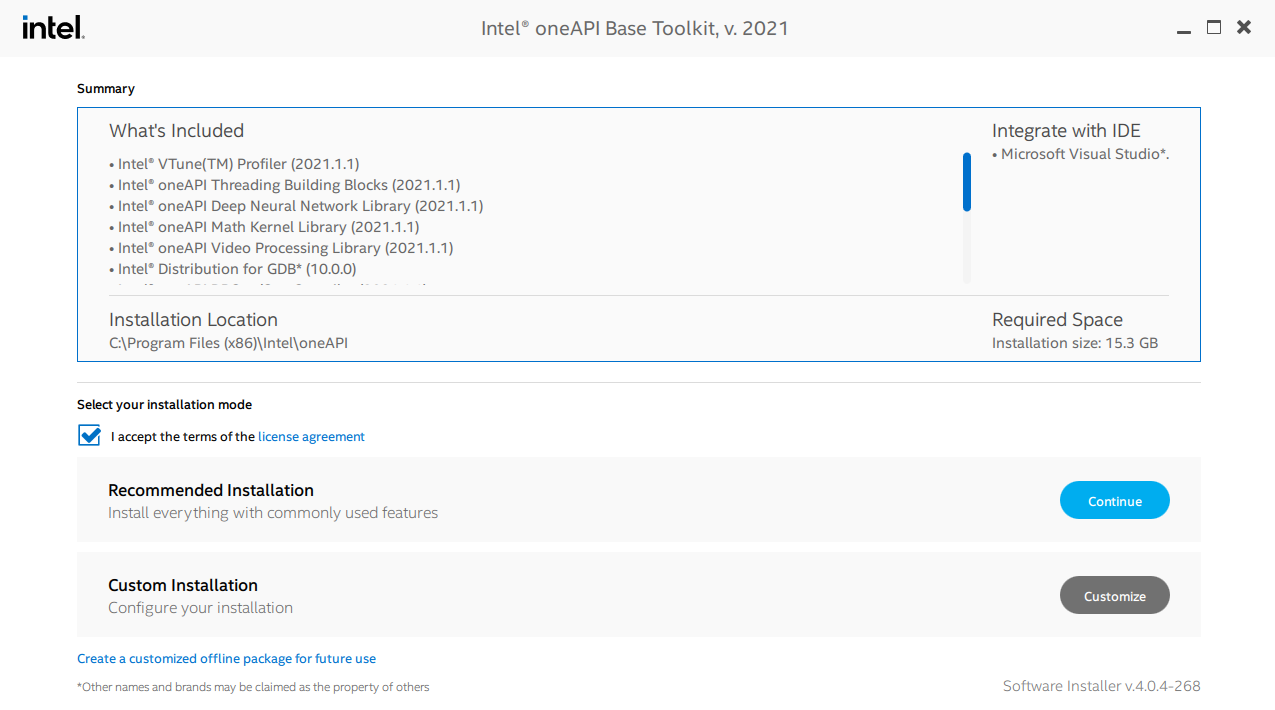
\includegraphics[width= \textwidth]{Figures/Proceso2C}
    \caption{First window that appears in the installation, follow the \textit{recommended installation} after accepting the \textit{terms of the license agreement}.}
    \label{fig:Proceso2C}
\end{figure}

\begin{figure}
    \centering
    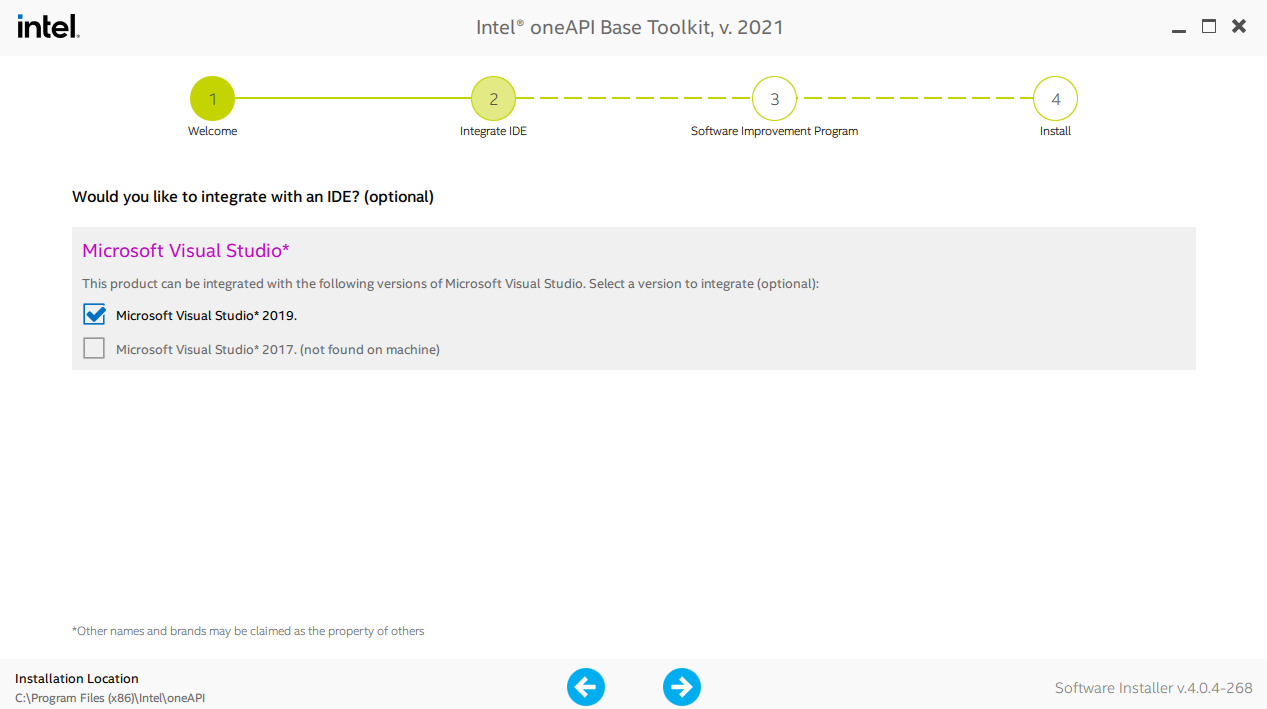
\includegraphics[width=\textwidth]{Figures/Proceso2D}
    \caption{Second step of the installation. Make sure the integration with your current version of Visual Studio is marked}
    \label{fig:Proceso2D}
\end{figure}

\begin{figure}
    \centering
    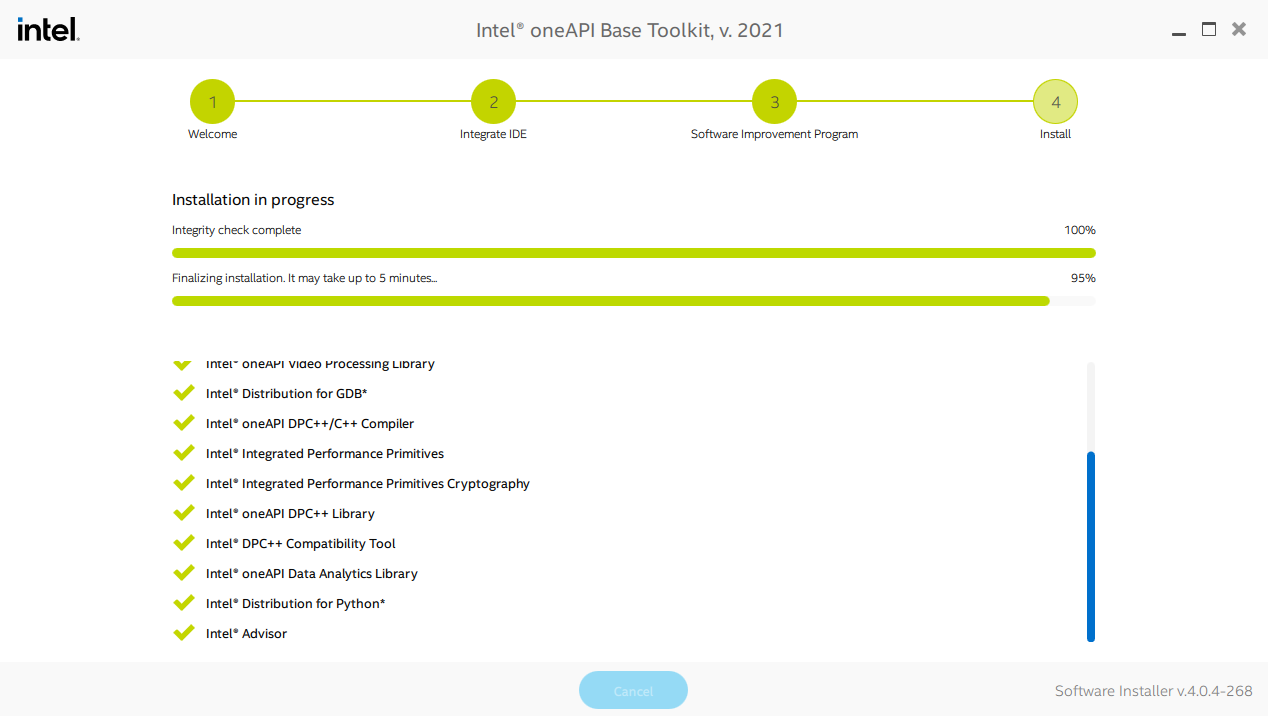
\includegraphics[width= \textwidth]{Figures/Proceso2E}
    \caption{Fourth step of the installation, wait until all the tools are installed.}
    \label{fig:Proceso2E}
\end{figure}



%\begin{IN}
%    \begin{itemize}
%        \item Please notice that Visual Studio \textbf{MUST be installed in the first place}. Do not continue with this installation if the IDE is not already installed in your computer.
%        \item The package used for the examples of this book is the \textit{version 2018 Update 3} of \textit{Intel\textregistered\hspace{0.05cm} Parallel Studio Cluster Edition}. However, you should install the latest version of the compiler offered by Intel\textregistered\hspace{0.1cm} in order to ensure the compatibility with the latest version of Visual Studio.
%    \end{itemize}
%\end{IN} 
%
%\begin{itemize}
%   	\item[a)] Downloading Intel\textregistered\hspace{0.05cm} Fortran Compiler with academic license:
%   	\begin{enumerate}
%   		\item We first go to the official website of Intel Developer Zone, click on the next url: \url{https://software.intel.com/en-us/qualify-for-free-software/student}.
%   		\item Click on \textit{Windows*} option of Intel\textregistered\hspace{0.05cm} Parallel Studio XE (Figure \ref{fig:ProcesoA}).
%   		\item We have to accept four options related to the use we are going to make of the software, we mark all of them and click on \textit{Accept} (Figure \ref{fig:ProcesoB}).
%   		\item Now we have to complete some personal information (Figure \ref{fig:ProcesoC}). It is important to write the institutional email in the box so we can receive the serial number for the installation and the confirmation email for the account we are creating.
%   		\item Click on \textit{Submit}.
%   		\item Fill in the form for the Intel Fortran \textit{Register an Account} (Figure \ref{fig:ProcesoCC}).
%   		\item Click on \textit{Register an Account}. We should receive a confirmation email now.
%   		\item This email has a download option and a Serial Number, keep this number somewhere in case you need to reinstall the tool in the future. 
%   		\item Click on download and select \textit{Intel\textregistered\hspace{0.05cm} Parallel Studio Cluster Edition for Windows* (all tools)} and \textit{version 2018 Update 3}.
%   		\item In order to avoid future problems during compilations we click on \textit{Full Package} in the Download Options. The file: \textit{parallel\_studio\_xe\_2018..... .exe} should be downloaded in your computer (Figure \ref{fig:ProcesoD}).
%   	\end{enumerate}
%
%   	\item[b)] Installing:
%   	\begin{enumerate}
%   		\item Execute the file \textit{parallel\_studio\_xe\_2018..... .exe}. 
%   		\item Click on \textit{Next} in the first step (Figure \ref{fig:ProcesoE}).
%   		\item Then we have to decide about consenting or not the collection of private information, choose your options.
%   		\item Click \textit{Next} once again.
%   		\item Now the installer shows warnings related to the needed modules (this step should not block the installation so we continue with the process), click on \textit{Next}. 
%   		\item Provide the Serial Number received in the email. 
%   		%\item The application finds automatically our license and it indicates that is going to %install tools for all Visual Studio versions found, which is what we need.
%   		\item The final step is clicking on \textit{Install} and waiting (it can be slow).
%   	\end{enumerate}
%\end{itemize}
%
%After the installation has finished we can start creating our Fortran projects and executing programs.
%
%\begin{figure}
%   	\centering
%   	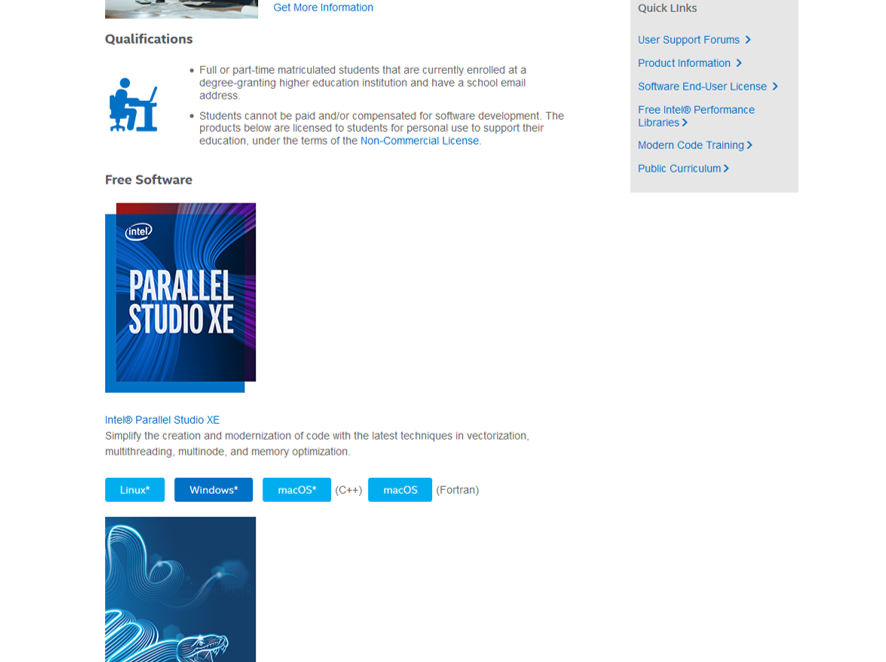
\includegraphics[width=0.8\textwidth]{Figures/ProcesoA}
%   	\caption{Different available options for the installation, choose Windows version.}
%   	\label{fig:ProcesoA}
%\end{figure}
%
%\begin{figure}
%   	\centering
%   	
\includegraphics[width=0.8  \textwidth]{Figures/ProcesoB}
%   	\caption{Select all the conditions and click on \textit{Accept}.}
%   	\label{fig:ProcesoB}
%\end{figure}
%
%\begin{figure}
%   	\centering
%   	
\includegraphics[width=0.7 \textwidth]{Figures/ProcesoC}
%   	\caption{Personal Information to complete in order to get the license.}
%   	\label{fig:ProcesoC}
%\end{figure}
%
%\begin{figure}
%   	\centering
%   	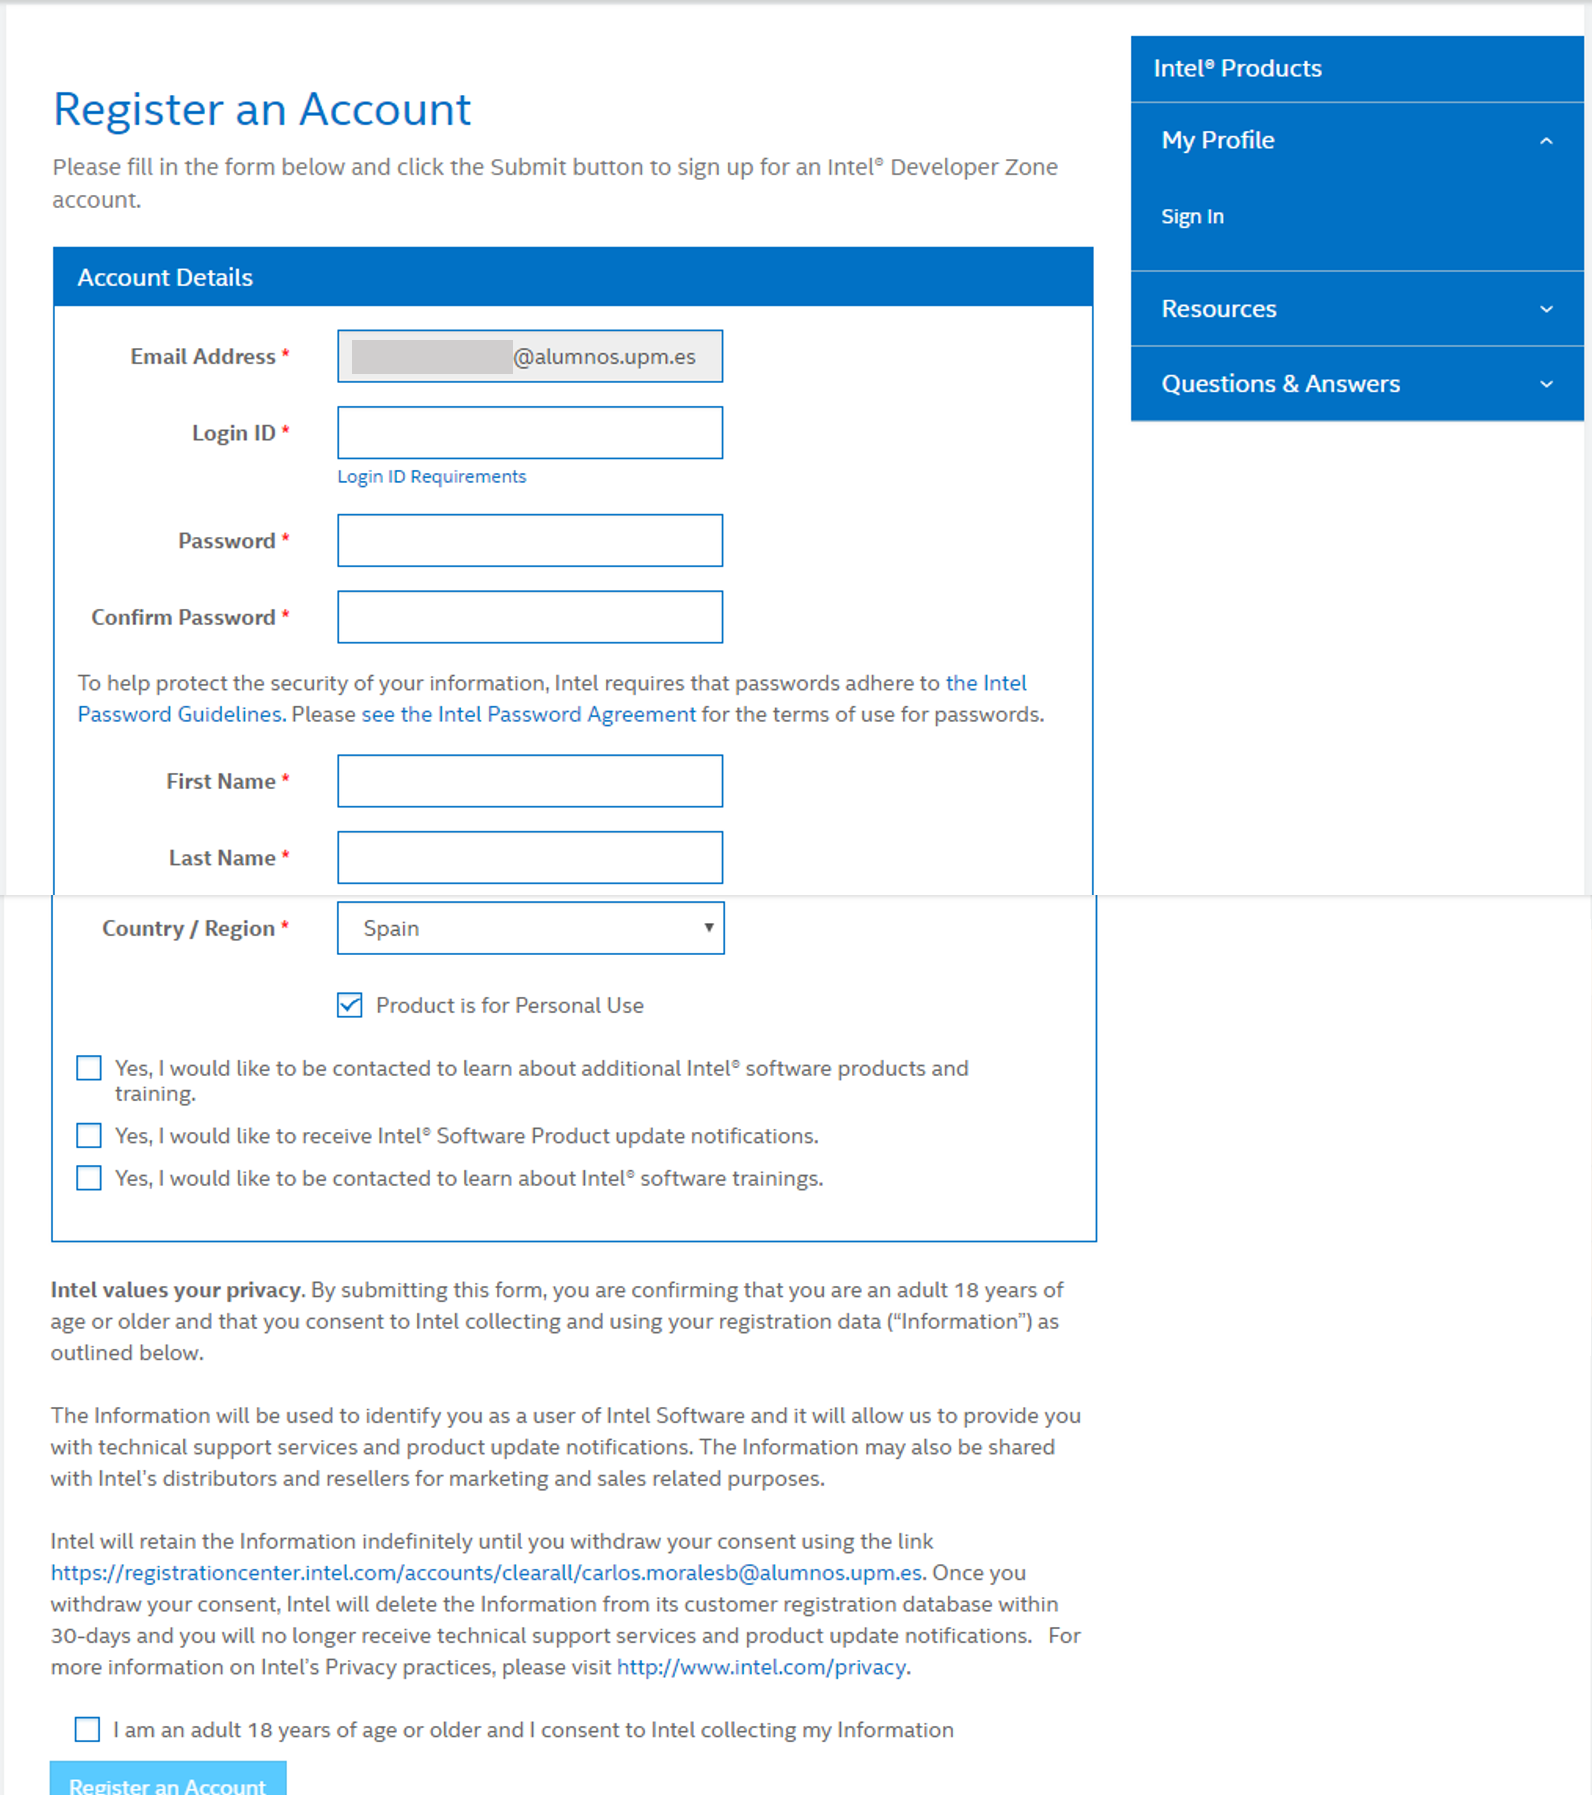
\includegraphics[width=0.6 \textwidth]{Figures/ProcesoCC}
%   	\caption{\textit{Register an Account} form in Intel Developer Zone, after filling in all the information click on \textit{Register an Account}.}
%   	\label{fig:ProcesoCC}
%\end{figure}
%
%\begin{figure}
%   	\centering
%   	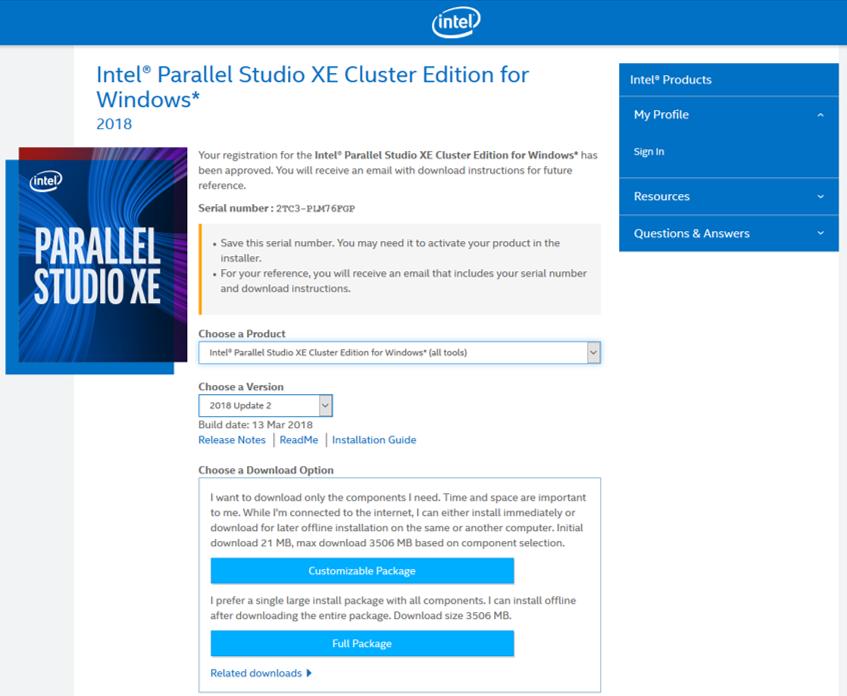
\includegraphics[width=0.6 \textwidth]{Figures/ProcesoD}
%   	\caption{Downloading page of Intel Parallel Studio, here, choose \textit{Intel Parallel Studio Cluster Edition for Windows* (all tools)} and \textit{version 2018 Update 3}.}
%   	\label{fig:ProcesoD}
%\end{figure}
%
%\begin{figure}
%   	\centering
%   	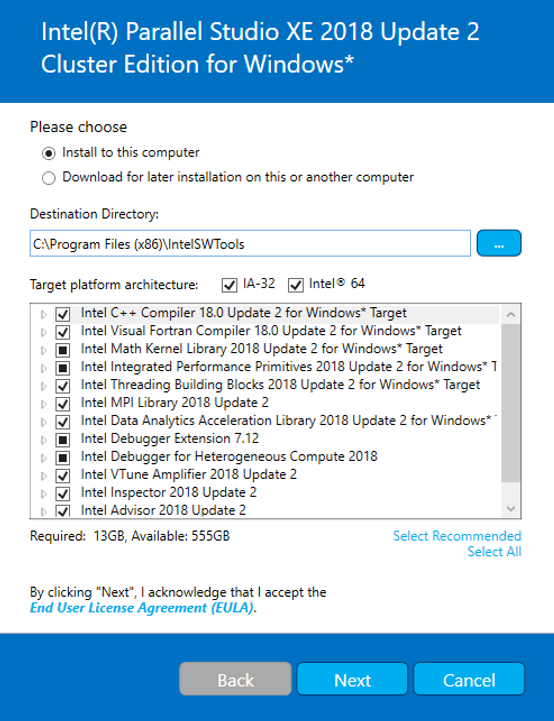
\includegraphics[width= 0.8\textwidth]{Figures/ProcesoE}
%   	\caption{These options are shown before installation. Select those marked here and click on \textit{Next}.}
%   	\label{fig:ProcesoE}
%\end{figure}



    \FloatBarrier
    \section{Create a Fortran project}

To create a Fortran project, proceed with the following steps: 

\begin{enumerate}
    \item Open your version of Visual Studio.
    \item Click on \textit{File/New/Project...} (Figure \ref{fig:Pro1}).
    \item In the \textit{Intel(R) Visual Fortran} menu select \textit{Console Application} and then click on \textit{Main Program Code}.
    \item Choose a name for the project (Figure \ref{fig:Pro2}). 
    \item Change the \textit{Location} of the solution, a directory will be created there.
    \item Choose the name of the solution, it does not have to be the same as the name of the project.  
    \item Select the option \textit{Create directory for solution}.
    \item Click on \textit{OK}.
\end{enumerate}


    \section{Compile, link and execute the ``Hello world" example}

In order to check that everything is correctly installed, we will run the easiest example. This is usually called the ``Hello world" example. This example is written automatically when we select 
\textit{Main Program Code}. This program opens the window console, writes the message ``Hello world" and after pressing the enter key, it closes the window console. 

If we want to execute this Fortran program, a translation to machine code must be done. This compiling and linking process is done automatically by Visual Studio by clicking the right button and is accomplished by the two following steps. Assuming the file is called ``p1'' for example, first the source file \texttt{p1.f90} is translated to an object code \texttt{p1.o} and then it is linked to other components to create an executable file: \texttt{p1.exe}. 
  
\newpage
To compile, link and execute the program follow the next steps:

\begin{enumerate}[nosep]
	\item Click on \textit{BUILD/Build solution} or click on the corresponding icon. The program is compiled and linked. 
	\item Click on \textit{DEBUG/Start Without Debugging} or click the corresponding icon. The program is executed. 
\end{enumerate}
    
%\lstinputlisting[language=Fortran, firstline=1, lastline=6]{Listing/Hello_world.f90}   

\begin{IN}
    More project/solution examples with Fortran language can be downloaded from: 
    
     \url{https://github.com/jahrWork/Visual-Studio-projects}.
\end{IN}


    \section{Include new projects and new files} \label{sec:Include}

Before learning how to include files in our project (whether new or existing ones), it is interesting to understand the difference between the logical order that is generated in our solution and the real order of the files stored in the hard drive. This concept has been introduced at the beginning of this guide and it is specially important for the case of Fortran. When our project grows, we include files and folders in the solution explorer in order to have all the source codes, images, libraries, etc. organized. However, each file can be stored anywhere in our hard drive, maybe in the folder of a different project/solution, in the desktop, in the cloud, etc. 

Think for example in a library that we use for different projects, it can be stored in a generic folder that is not related to the projects at all. It is responsibility of the programmer to have also the files organized in the computer in order to avoid problems when linking the project (e.g avoiding changes of files location). As an example see the Figure \ref{fig:Config2}, we see in the Solution explorer a large number of folders but if we open the project we find that all the source codes are stored in the same folder (including also the libraries and modules of dislin).

On one hand, in the case of Fortran, in the solution explorer we find three folders by default: \textit{Source}, \textit{Resource} and \textit{Header Files}. We typically use the Source folder for all the source codes written for the project while the other two are empty. Create the most appropriate structure inside \textit{Source} folder (by creating new folders for example) and organize the project. The libraries and modules can also be included there. 

On the other hand, in the hard drive the structure is different, choose the most comfortable for your purposes. Apart from the \texttt{.sln} and the \texttt{.suo} files in the solution folder and the \texttt{.vfproj} file in the project folder (all essential for the project), we find the folders associated to the results of the build and compilation processes. If we build the project in the Release configuration, a \texttt{Release} folder appears with the \texttt{.obj} and \texttt{.mod} files, the executable, etc. If it is built in Debug mode, the same happens with a \texttt{Debug} folder. We suggest to create a \texttt{sources} folder inside the project path and store there all the \texttt{.f90} real files with the source code.

We can check in the solution location that after creating the solution and project, a \texttt{.sln} file, a folder with the name of the project and a \texttt{.vfproj} file inside have appeared. If the Solution is already created and we just want to open it we can double click on the \texttt{.sln} file or click on \textit{File/Open/Project/Solution...} in the IDE and look for our \texttt{.sln} file. 

\textbf{Include another project} in that solution:
\begin{enumerate}[nosep]
    \item Click on \textit{File/New/Project...}.
    \item In the \textit{Intel(R) Visual Fortran} menu select \textit{Console Application} and then click on \textit{Empty Project}.
    \item Write the name of the new project.
    \item In \textit{Solution} select the option \textit{Add to solution}.
    \item Click on \textit{OK}.
    \item Before closing Visual Studio do not forget to click on \textit{Save All}.
\end{enumerate}
    
\begin{figure}[h]
    \centering
    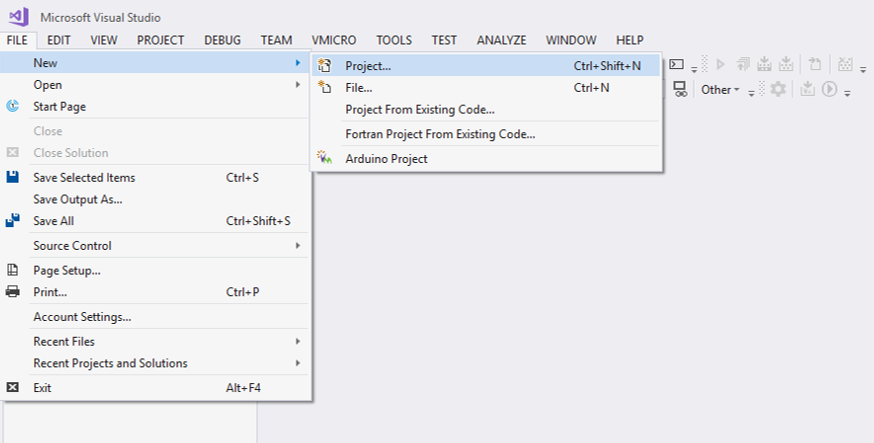
\includegraphics[width=\textwidth]{Figures/Pro1}
    \caption{First step in order to create a solution with a Fortran project.}
    \label{fig:Pro1}
\end{figure}

\begin{figure}[h]
    \centering
    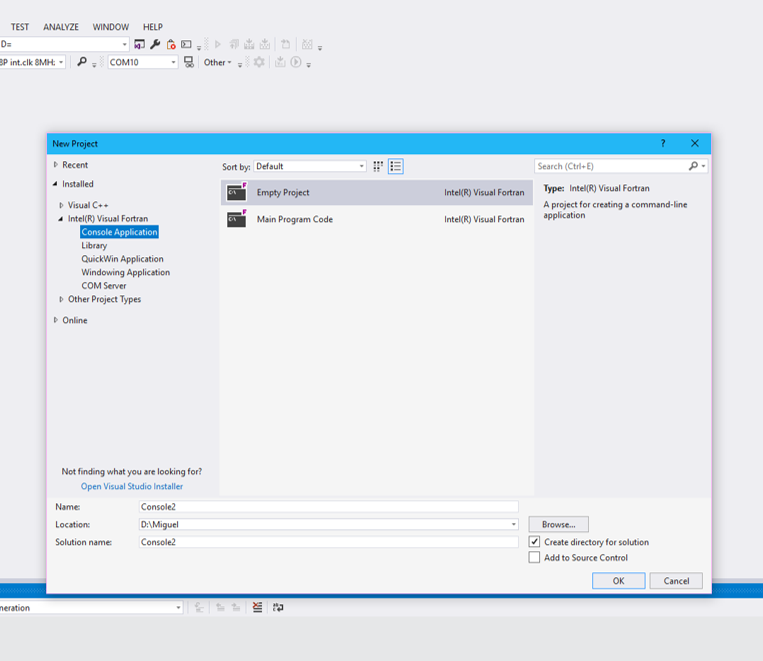
\includegraphics[width= \textwidth]{Figures/Pro2}
    \caption{Second step in order to create a solution with a Fortran project.}
    \label{fig:Pro2}
\end{figure}

\label{Including}\textbf{Including files} in a project is easy:
\begin{enumerate}[nosep]
    \item Right click on the name of the project (in the solution explorer).
    \item Click on \textit{Add}.
    \item Click on \textit{New Item...} if you are going to start from scratch (or click in \textit{Existing Item...} if you add it from an existing one).
    \item Click on \textit{Fortran Free-form File (.f90)}.
    \item Write the name of the file.
    \item Click on \textit{Add}.
\end{enumerate}

\begin{IN}
    \begin{itemize}     
        \item By default, the created file appears in the source folder but we can grab and drop it in the root location of the project so it appears in the same level as Source, Resource and Header folders. 
        \item For those files that we include in our project from a different location (not the folder where we store all the project), we have to bear in mind that Visual Studio will \textbf{look for it in the original location the next time} and thus we cannot change location. A better option would be saving a copy in our project folder and include it from there.
    \end{itemize}
\end{IN}



    \FloatBarrier
    \section{Configuring compilation options}
    
In the section \ref{sec:ConfigVS} we have seen how to configure general VS settings, however, notice that those options are not related to the \textbf{Fortran project configuration}. For each project inside our solution (or any project we create from now on) we have to define some compilation properties. Actually, it is possible to define some properties for every \textbf{individual source code file} (by clinking right button on the name of the file and clicking on properties) but we are going to treat here some of the properties that involve \textbf{the whole project}.

With the project opened and selected in the solution explorer we have to click on \textit{Project/Properties}, the changes we make now will only affect to the chosen project. First of all check in this window that the \textit{Configuration} selected is the Active one, which means, if you are running the application in Release mode, then change the properties of the Release mode (and the same if you are running the program in a different configuration). A change applied only to the Debug mode won't affect to the rest of configurations. The configuration (or mode) that you are modifying in the window opened can be checked in the top-left part of the window itself. 

\begin{IN}
    \begin{itemize}  
        \item If we have selected a specific file in the solution explorer (and not the whole project) the properties shown in the window opened are the \textbf{individual file properties}. Hence, take care of what is marked in the solution explorer.
        
        \item In addition, notice that a change in the properties of the project will change all internal files \textbf{except those properties of files that we have changed individually}. 
        
        For example, if we mark \textbf{\textit{8 (/real\_size:64)}} in \textit{Fortran/Data/default Real KIND} in a \texttt{example.f90} file and we change the same option in the project configuration (let's say to \textbf{\textit{16 (/real\_size:128)}}), all files are modified but \texttt{example.f90} does not. What's more, a red spot appears in the symbol of the file in the solution explorer notifying this condition. Furthermore, if the option does not have the compiler's default value, the value itself appears in bold in the configuration window.
    \end{itemize}
\end{IN}

Now let's take a look at some important compiler options that can be found in the window \textit{Project/Properties}:

\begin{enumerate}[nosep]
    \item Default Real KIND
    \item Stack
    \item Heap arrays
    \item Automatic Reallocation
    \item Traceback Information
    \item Runtime Error Checking
    \item Treat Warnings As Errors
    \item Warn For Non-standard Fortran
    \item Compile Time Diagnostics
\end{enumerate}



\newpage
\begin{enumerate}
    
    %%%%%%%%%%%%%%%%%%%%%%%%%%%%%%%%%%%%%%%%%%%%%%%%%%%%%%%%%%%%%%%%%%%%%%%%%%%%%%%%%C
    \item In \textit{Fortran/Data/\textbf{Default Real KIND}} we can change the default value to ``8 (/real\_size:64)''. Then, when we write in our code 
    
    \textcolor{black}{\texttt{real :: x}}  
    
    the default kind of the x will be 8 bytes (double precision) and we do not have to specify 
    
    \texttt{real(kind=8) :: x} 
    
    every time we declare a variable in double precision. When we use this trick, we get used to write only \texttt{real :: x} in our programs and not mix different precisions in the same code. 
    
    Using this compilation option, when we want to run our program with simple precision, we just have to change the value and the whole program will be executed with simple precision. The following example shows both ways of executing the same program and demonstrates that the results can be different depending on the compiler options. \label{Configuration1}
    
    Execute the following code changing the \textit{Default Real KIND} value in the compiler options, first with the value by default (simple precision) and then forcing the code to be executed in double precision. \vskip \baselineskip
    
    \lstinputlisting[language=Fortran, firstline=1, lastline=24]{Listing/ExManual2.f90}

    In the first case you are going to obtain this:
    
    \begin{verbatim}
Declaration of x with - real(4):: x
Maximum value  3.4028235E+38
Minimum value  1.1754944E-38
Round_off  1.1920929E-07
Significant digits           6
Declaration of y with - real :: y
Maximum value  3.4028235E+38
Minimum value  1.1754944E-38
Round_off  1.1920929E-07
Significant digits           6
    \end{verbatim}
    
    While in the second one, the results are:
    
    \begin{verbatim}
Declaration of x with - real(4):: x
Maximum value  3.4028235E+38
Minimum value  1.1754944E-38
Round_off  1.1920929E-07
Significant digits           6
Declaration of y with - real :: y
Maximum value  1.797693134862316E+308
Minimum value  2.225073858507201E-308
Round_off  2.220446049250313E-016
Significant digits          15
    \end{verbatim}
    
\begin{IN}
    \begin{itemize}
\item Notice how in both cases the \verb|x| is a simple precision real number since we are forcing the program to declare this variable as \verb|kind=4|. Then, the upper limit for this variable is around \texttt{E+38} as the \verb|huge(x)| function returns, the lower limit is around \texttt{E-38} according to \verb|tiny(x)| function and we can trust the first 6 significant digits of the number (\verb|epsilon(x)| calculates this value). 

\item However, the behaviour of the \verb|y| is really different. In the declaration of the variable we have not specified the kind of the real variable. As said before, in the first execution (\textit{Default Real KIND} 4), the compiler treats \verb|y| as simple precision and in the second execution (\textit{Default Real Kind 8}) the variable is treated as double precision. Hence, the limits for \verb|y| in the second case are those related to double precision (\texttt{E+308}, \texttt{E+308} and 15 significant digits). In conclusion, the same code can return different results depending on the compilation options.
    \end{itemize}
\end{IN}   
    

    %%%%%%%%%%%%%%%%%%%%%%%%%%%%%%%%%%%%%%%%%%%%%%%%%%%%%%%%%%%%%%%%%%%%%%%%%%%%%%%%%C
    \item \textbf{Stack Overflow} can occur in our software for many reasons. It happens when the stack memory overflows and occupies other memory regions, then the stack pointer exceeds the stack bound \citep{stack} (concepts like call stack can be found in \citep{stack2}). Since the problem is to allocate more memory on the stack than the maximum that fits (too large local arrays or infinite recursion for example) one solution is to extend the size of the stack. We can change the configuration by clicking on \textit{Linker/Command Line/Additional Options:} and writing ``/STACK:100000000''.
    
    %%%%%%%%%%%%%%%%%%%%%%%%%%%%%%%%%%%%%%%%%%%%%%%%%%%%%%%%%%%%%%%%%%%%%%%%%%%%%%%%%C
    \item \textbf{Heap allocation} is another method to avoid stack overflow in our programs. The heap is one of the three memories used by a Fortran application, it is dynamically allocated, bigger than the Stack in size but also slower. However, if your program needs from large automatic arrays (those whose size is defined by routine arguments) or makes arithmetic with large arrays (temporary arrays are normally stored in the stack) it can be a good idea to automatically store those arrays in the Heap, instead of stack. In order to do that click on \textit{Fortran/Optimization/Heap Arrays} and write a value in kilobytes for the minimum temporary/automatic array size to be allocated in heap. If \texttt{0} is written, then all those arrays are affected. Notice that writing \textit{/heap-arrays0} in \textit{Fortran/Command Line/Additional Options} is another way to do the same. 
    
    %%%%%%%%%%%%%%%%%%%%%%%%%%%%%%%%%%%%%%%%%%%%%%%%%%%%%%%%%%%%%%%%%%%%%%%%%%%%%%%%%C
    \item In \textit{Fortran/Command Line/Additional Options:}, in order to enable \textbf{automatic reallocation}, write ``/assume:realloc\_lhs''. This option decides if using current Fortran Standard rules or old Fortran 2003 rules in relation to the automatic reallocation, which is described as:
    
    \begin{center}
        \begin{minipage}{0.7\linewidth}
            \vspace{5pt}
            {\small
                ``Tells the compiler that when the left-hand side of an assignment is an allocatable object, it should be reallocated to the shape of the right-hand side of the assignment before the assignment occurs. This is the current Fortran Standard definition. This feature may cause extra overhead at run time. The option standard-realloc-lhs has the same effect as assume realloc\_lhs.''
            }
            \begin{flushright}
                (\url{https://software.intel.com/en-us/node/678222})
            \end{flushright}
            \vspace{5pt}
        \end{minipage}
    \end{center}



    %%%%%%%%%%%%%%%%%%%%%%%%%%%%%%%%%%%%%%%%%%%%%%%%%%%%%%%%%%%%%%%%%%%%%%%%%%%%%%%%%C
    \item In \textit{Fortran/Run-time} the option \textbf{\textit{Generate Traceback Information}} is by default deactivated. Set it as \textit{Yes} so extra information will be placed in the object files and in the case of appearing a severe error in the run time, you will be capable of locate the source of error because source file, routine name and line number correlation will be displayed. This function is independent of the Debug option.
    
    %%%%%%%%%%%%%%%%%%%%%%%%%%%%%%%%%%%%%%%%%%%%%%%%%%%%%%%%%%%%%%%%%%%%%%%%%%%%%%%%%C
    \item In the same section, \textit{Fortran/Run-time}, fix the option \textbf{\textit{Runtime Error Checking}} to \textit{All} so the compiler checks at run time all the available conditions. These conditions are for example related to pointers (check if some allocatable objects are not allocated) or uninitialized variables. Some conditions in the code that could be ignored by the compiler, in this case are considered as Warnings and the compilation shows them. Then, it forces the programmer to make a clean code and take control of those inappropriate conditions. 
    
    %%%%%%%%%%%%%%%%%%%%%%%%%%%%%%%%%%%%%%%%%%%%%%%%%%%%%%%%%%%%%%%%%%%%%%%%%%%%%%%%%C
    \item In the section \textit{Fortran/Diagnostics} activate \textbf{\textit{Treat Warnings As Errors}}. This option changes some Warnings to Errors so the compilation will fail until they are solved. This function helps to maintain a clean code and avoids to accumulate bugs in a program. Even when those warnings could let the program be compiled, they can also be conceptual mistakes and they can become a problem if a lot of ignored warnings are accumulated in the projects.
    
    %%%%%%%%%%%%%%%%%%%%%%%%%%%%%%%%%%%%%%%%%%%%%%%%%%%%%%%%%%%%%%%%%%%%%%%%%%%%%%%%%C
    \item In the same section, \textit{Fortran/Diagnostics}, the option \textbf{\textit{Warn For Non-standard Fortran}} makes the compiler to return warnings when there are language elements that are not contained in the Fortran standard. These standard warnings do not affect compilation but they help the programmer to modernize the programming style, ensure that other programmers understand the code, comply with common rules and avoid problems with different compilers. In our case, we want to be adapted to the Fortran 2008 standard so fix that value in the compilation option.
    
    %%%%%%%%%%%%%%%%%%%%%%%%%%%%%%%%%%%%%%%%%%%%%%%%%%%%%%%%%%%%%%%%%%%%%%%%%%%%%%%%%C
    \item Set the option \textit{Fortran/Diagnostics/\textbf{Compile Time Diagnostics}} to \textit{Show All} and the compiler will warn about a pile of interesting conditions to consider. For example, it will issue information about: variables declared in the code but not used after that, source code lines that exceed the maximum column width or statement functions that are never called in the program. 

\end{enumerate}




\newpage
\FloatBarrier
    \section{Configuring a graphic library: DISLIN}
    
\textbf{DISLIN} is a plotting library for Fortran and C languages created by the Max Planck Institute (MPS). It is a high-level plotting library for displaying data and allows a quick plot of results when we are making a lot of tests with the code or debugging (graphic debugging) our program. It can be called from the main program or subroutines and ``contains routines and functions for displaying data as curves, bar graphs, pie charts, 3D-colour plots, surfaces, contours and maps''. In order to use DISLIN libraries in our project, we have to add some files first. Follow these steps: 

\begin{enumerate}
     \setlength\itemsep{0.0cm}
    \item Download the DISLIN distribution package required for our machine. Open the web:
    
    \url{https://www.dislin.de/win64.html} 
    
    and choose Intel Fortran compiler package. 
    
    \item  Unzip the downloaded file and look for: 
    
    \texttt{disifl\_d.lib} and \texttt{dislin\_d.f90}
     
    It is assumed that our calculations are done in double precision and that is why double precision files (\texttt{*\_d.lib, dislin\_d.f90}) are selected. 
     
    \item Create a folder named DISLIN and locate those files on it. 
    
    \item Include this folder and all the items in our Visual Studio project following the process mentioned in section \ref{Including}.
    
    \item To avoid errors configure the project to: \textit{Platform: x64} and \textit{Configuration: All Configurations} by clicking with right button in your solution (in the solution explorer) and opening:
    
        \textit{Properties/Configuration Properties}. 
        
    \item Also, in the project properties: 
    
    \textit{Properties/Fortran/Data/Default real kind} to 8. 
    
    \item \textit{Properties/Fortran/Libraries/} : Multithreaded.
     
    \item \textit{Properties/Linker/Input/Additional Dependencies} : user32.lib, gdi32.lib. 
        
    \item Revise \textit{IgnoreDefaultLibraryNames} : empty, none.  
    
\end{enumerate}     
    
%    
%     (Figure \ref{fig:Config5}). Open the project property pages and check that in \textit{Fortran/Libraries/Runtime Library} is written 
%``Multithread DLL (/libs:dll /threads)''.
%    
%    \item Configure the project to avoid duplications. Open the project property pages in \textit{Linker/Input/Ignore Specific Library} and 
%write in the space reserved: ``LIBCMT;libifcoremd''. A detailed image of the configuration process is shown in Figure \ref{fig:Config5}.
%    
%    \item Once the configuration process has been finished, the solution explorer looks like the example of Figure \ref{fig:dislin}. 
%Remember that a complete dislin manual can be found in the dislin web page.  
 


Now our dislin example should work, take note of the subroutines used in the plotting example below in order to use it in future codes. The example allows to plot a sine graph in a very simple way. It is advisable to write a \texttt{read(*,*)} line at the end of the program to avoid that the command line gets closed after finishing. \vspace{0.5cm}

\lstinputlisting[language=Fortran, firstline=1, lastline=30]{Listing/Graph.f90} 

\begin{IN}
    In case that you comment the \texttt{use dislin} statement that enables the use of DISLIN libraries (because you are not going to use it for example) do not forget to reverse last two steps of the DISLIN configuration. A list of errors could appear while building the code if you do not change the configuration. 
\end{IN}


%\begin{figure}
%    \centering
%    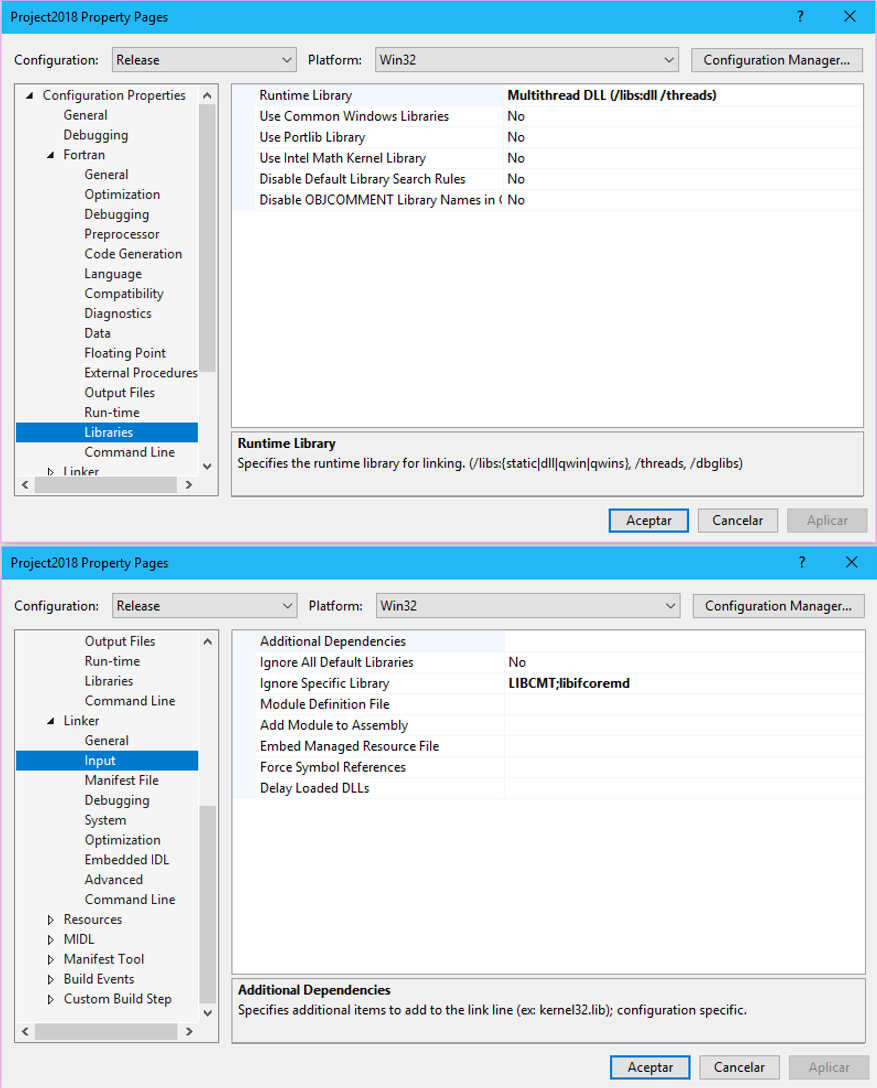
\includegraphics[width= \linewidth ]{Figures/Config5}
%    \caption{Necessary configuration for the Project Properties in order to make the program work with DISLIN, the fields to change are 
%\textit{Runtime Library} and \textit{Ignore Specific Library}.}
%    \label{fig:Config5}
%\end{figure}
%
%\begin{figure}
%    \centering
%    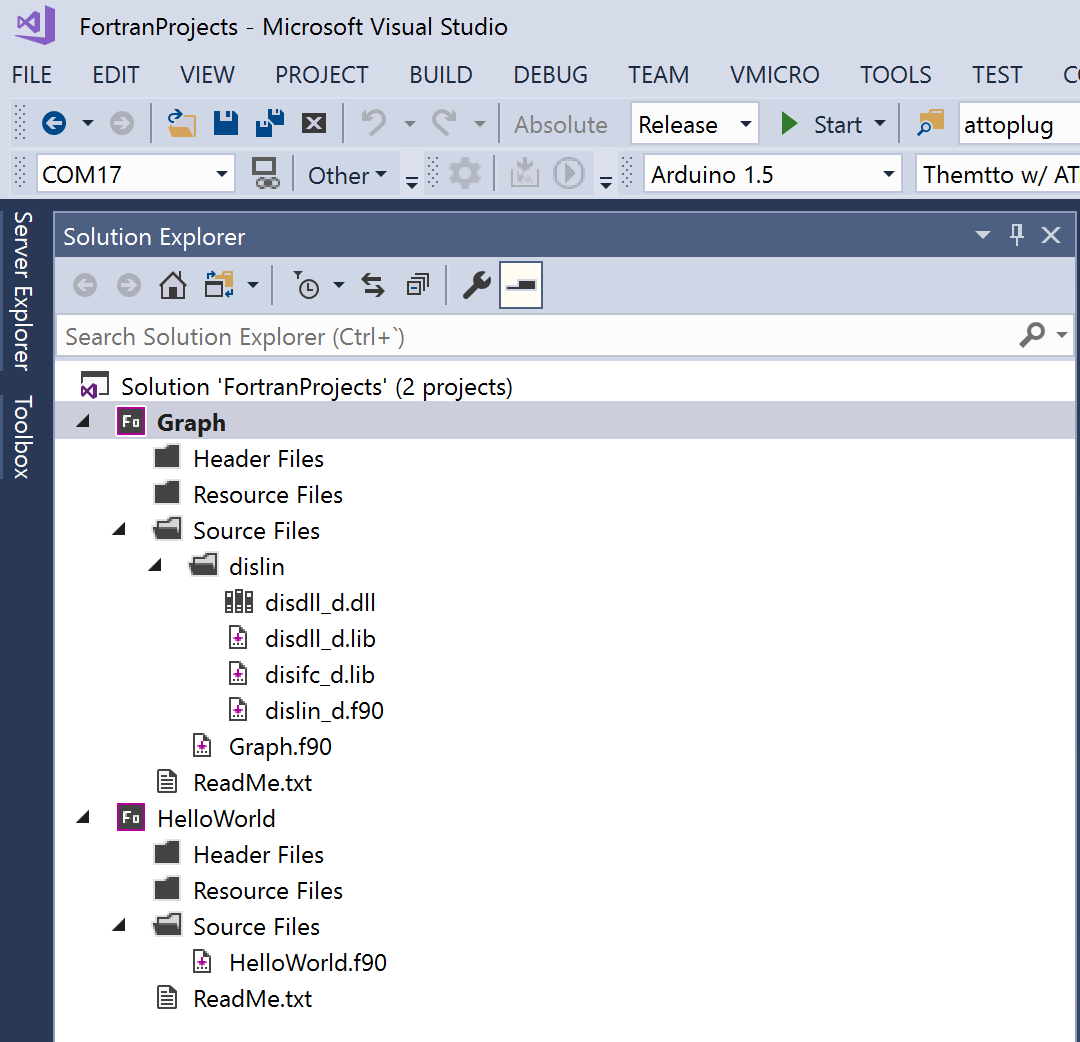
\includegraphics[width= \linewidth ]{Figures/dislin}
%    \caption{Solution explorer for the project Graph showing the inclusion of dislin libraries and \textit{dislin\_d.f90} interfaces.}
%    \label{fig:dislin}
%\end{figure}



    \section{Fortran FAQ}

In this section some general concepts and good practices are going to be explained through Frequently Asked Questions.

\begin{enumerate}[nosep]
    \item What are Release and Debug execution modes?
    \item What are Compile, Build and Start without debugging?
    \item What are Static and Dynamic libraries? How can I create a \texttt{.lib} file?
    \item What should I know about files and formats in Fortran language?
\end{enumerate}

\begin{enumerate}
    
    %%%%%%%%%%%%%%%%%%%%%%%%%%%%%%%%%%%%%%%%%%%%%%%%%%%%%%%%%%%%%%%%%%%%%%%%%%%%%%%%%C
    \item \textbf{What are Release and Debug execution modes?} 
    
    Release and Debug are two possible modes for executing our program, each of them has its own default configuration that allow us to build and run the code in a different way. We can create more modes with different configurations for the solution or for the project. For example, we could create one mode where the option \textit{Default Real KIND} of Fortran compiler is 4 and other where it is 8. In the first one a variable declared as a real number will be considered of simple precision by default, in the second case it will be treated as a double precision real number. By changing between both modes, we would run the code with the two configurations. In order to define these modes we can access the Configuration Manager by clicking on \textit{Build/Configuration Manager} or by deploying the selector of Configuration (where the mode \textit{Release} or \textit{Debug} are shown). There we can create new modes or edit those we have. Once a mode is selected, the configuration can be modified in the properties page of the project (click with the right button in the name of the project and click on \textit{Properties}). 
   
    Regarding the Debug mode, it will allow you to run the code without turning on the optimiser. A lot of information will be included in the build files so we can check our program step by step, it can be useful for example for fixing bugs. However, if we are developing Numerical Simulations and related programs, we will use another kind of debugging: graphic assisted debugging. Checking errors in the code starts with the printing of results and the validation of the program module by module. That is why we typically include Dislin libraries in our program, to check results quickly and decide if we have programmed correctly our simulation, later we will save the numerical results in order to plot them with another tool. 
    
    %%%%%%%%%%%%%%%%%%%%%%%%%%%%%%%%%%%%%%%%%%%%%%%%%%%%%%%%%%%%%%%%%%%%%%%%%%%%%%%%%C
    \item \textbf{What are Compile, Build and Start without debugging?}
    
    We have seen what Debug and Release modes are and we now understand why one of the first IDE configurations to make is changing the command that executes the program, from the \textit{Start with Debugging} to this one (see section \ref{StartwD}). This command goes directly to the execution of the code using the Release mode (or the selected one, but not debugging). However, we are going to take a closer look at the different options mentioned.
    
    \textbf{Compile:} Once our project is created inside a solution and the first codes are written, we want to compile the program file by file in order to check that everything is correct. In this step the compiler comes into play, it checks and warns us about all the errors that exists in the program. In order to compile your piece of code open its file and click on \textit{BUILD/Compile} in the IDE. You can also press \texttt{Ctrl+F7} or click in the following symbol (that should be in your toolbars\footnote{If you can not see the symbol go to the section \ref{sec:Shortcuts} and modify the aspect of your IDE to show all the interesting shortcuts.}). Notice that you are compiling only the file opened and not the whole project.
    
    %\raisebox{-\mydepth}{\fbox{
\includegraphics[height=2\myheight]{Figures/CompileSymbol}}}
    \begin{figure}[H]
        \centering
        
\includegraphics[width= 0.1\textwidth]{Figures/CompileSymbol}
        %\caption{Example of \textit{Intrinsic Quick Info}.}
        %\label{fig:Commands6}
    \end{figure}
    
    \textbf{Build:} With this command Visual Studio will compile and link the source files of your program. You can build only the project that you have opened or you have selected in the Solution Explorer with the option \textit{BUILD/Build ``Name of the project''} or clicking in the symbol 
    
    %\raisebox{-\mydepth}{\fbox{
\includegraphics[height=2\myheight]{Figures/Build1Symbol}}}
    \begin{figure}[H]
        \centering
        
\includegraphics[width= 0.1\textwidth]{Figures/Build1Symbol}
        %\caption{Example of \textit{Intrinsic Quick Info}.}
        %\label{fig:Commands6}
    \end{figure}
    
    You can also build the whole solution, with all the projects involved, by clicking in \textit{BUILD/Build Solution} or clicking in the symbol 
    
    %\raisebox{-\mydepth}{\fbox{
\includegraphics[height= 2\myheight]{Figures/Build2Symbol}}}
    \begin{figure}[H]
        \centering
        
\includegraphics[width= 0.1\textwidth]{Figures/Build2Symbol}
        %\caption{Example of \textit{Intrinsic Quick Info}.}
        %\label{fig:Commands6}
    \end{figure}
    
    In this case it does not matter which project you have selected since the whole solution is going to be compiled and linked. 
    
    \begin{IN}
        \begin{itemize}
            \item \textbf{Build} command is going to perform an incremental build. This means that if Visual does not think it needs to build anything in the project (because the files did not changed since the last build), then it won't build anything. It is going to compile only the files that have changed and hence, the process is quicker. This is the most common used command to build our program. If here is no changes in the files, and you try to build everything two times, a message will appear saying that all the code is up-to-date.
            
            \item If \textbf{Clean} command is used, whether \textit{BUILD/Clean ``Name of the project''} or \textit{BUILD/Clean Solution}, Visual Studio is going to delete all the compiled and intermediate files that exist (only for one project or the whole solution respectively). Then, if you want to build the program again, we have to wait for all the files and codes to be compiled and linked. We can use this if you are interested in starting a new compilation of all the source files. When you clean all the solution, the projects involved are cleaned one by one.
            
            \item \textbf{Rebuild} option, whether it is for only one project or the whole solution, will clean and then build the project/solution from scratch. The difference between using this and clicking first  in Clean and later in Build is that Rebuild (in the case of a solution) will clean and build one project, later clean and build another one, etc. instead of cleaning all of them and then building all the solution.
        \end{itemize}    
    \end{IN}
    
    \textbf{Start Debugging/Start without Debugging:} When you want to execute your program the command \textit{Start without Debugging} is used. It \textbf{saves} the modified files, \textbf{compiles}, \textbf{links} and \textbf{executes} all the project selected in the Solution Explorer. In other words, it makes all the previous steps necessary to execute the program. Notice that it uses the build option (compile and link) so nothing will change if there is no changes in the files. 
    
    There are two options for this task; attach the debugger to the execution of the application or not. In the first case you will be able to pause the execution by breakpoints or use debugging tools such as Watch Window or Diagnostic Tools. However, if you just want to run your application and see the results, it is not necessary to use this integrated debugger, there are different ways of performing a debugging of the code when needed. 
    
    If \textit{Start without Debugging} option is used Visual Studio will launch your application without attaching the Debugger. Both ways of executing the code can be found in the menu \textit{DEBUG} of the IDE and more specifically the option \textit{without Debugging} can be found clicking on \textit{DEBUG/Start without Debugging}, pressing \texttt{Ctrl+F5} or pressing the following icon of your toolbars\footnote{See previous footnote}. 
    
    %\raisebox{-\mydepth}{\fbox{
\includegraphics[height=2\myheight]{Figures/StartSymbol}}}
   \begin{figure}[H]
        \centering
        
\includegraphics[width= 0.1\textwidth]{Figures/StartSymbol}
        %\caption{Example of \textit{Intrinsic Quick Info}.}
        %\label{fig:Commands6}
    \end{figure}
    
	
	%%%%%%%%%%%%%%%%%%%%%%%%%%%%%%%%%%%%%%%%%%%%%%%%%%%%%%%%%%%%%%%%%%%%%%%%%%%%%%%%%
	\item \textbf{What are Static and Dynamic libraries? How can I create a \texttt{.lib} file?} \label{sec:Library}
	
	Let's say we have some modules already validated and we want to create a library with them, the first thing to do is to decide the kind of library to use. 
    
    On one side, in a \textbf{Static Library} the code written is compiled and located inside the executable file once it is created, we could go to another computer and run that executable file (the program) without problems. Then, we have a fast program since it has all the necessary code inside and does not have to look for part of the program ``outside''. However, it also has some disadvantages, for example programs become heavier and if we find a bug in the library, we will have to recompile the whole program. 
	
	On the other side, \textbf{Dynamic libraries} are not stored in our executable file, they are added as an external file. It becomes a lighter program and fixing bugs is easier as soon as it is repaired for all programs once we change just one file. However, we have to drag all libraries when moving the executable to another computer and the execution will be slower because of the search that the program has to perform when it needs those codes. 
    
    In conclusion, both have advantages and disadvantages and one or the other will be used depending on the situation. Each of them is created, compiled and linked in a different way. Let's see how to create a static library and a full program that uses the library through an example:
	
	\begin{enumerate}
        
		\item Create a new solution (or recycle one of the previous sections). Then, in this solution, create a new project as it is explained previously in this chapter. This project will contain the call to the subroutines stored in the library. Do not forget to choose a proper name for the project.
        
		\item Include an empty file called \texttt{ExampleManual2.f90} in the project and copy the following code:
	    
        \vspace{0.5cm}
		\lstinputlisting[language=Fortran, firstline=1, lastline=16]{Listing/ExampleManual2.f90}
        
        Notice that the program (called \verb|ExampleManual2|) is going to \verb|use| a module named \verb|ModuleExample| and is going to \verb|call| to the subroutines \verb|HelloWorld| and \verb|WritePI| contained in that module. 
		
		\item Now create a new project in the same solution (it could be done in a different solution), this time with kind \textit{Static Library}. In order to do that click on:
        
        \textit{File/New/Project.../Installed/Intel(R) Visual Fortran}
        
        and then: 
        
        \textit{Library/Static Library}
        
        Take care of choosing a proper name for the library project (it will be the name of the \texttt{.lib} file), in this case let's use the same name as the module \texttt{ModuleExample.lib}.
        
		\item Add to this Library project an empty source file called \texttt{ModuleExample1.f90} and paste the next example code, this will be the module code stored in our library:	
        
        \vspace{0.5cm}
        \lstinputlisting[language=Fortran, firstline=1, lastline=29]{Listing/ModuleExample.f90}		
		
		\item Then save all and set the library project as startup project (click with the right button on its name in the solution explorer and click on \textit{Set as StartUp Project}). Compile the file \texttt{ModuleExample.f90} and build the whole library project in the Release mode. Check that \texttt{ModuleExample.lib} and \texttt{ModuleExample.mod} appear in the Release folder of the project.
        
		\item Add to the main project both library files with the Solution Explorer in the \textbf{Source folder} using \textit{right click in the project name/Add/Existing Item.../} and looking for the files (see section \ref{sec:Include}).
        
        There are \textbf{two options}: in the \textbf{first one} you can copy both files in the folder of the main project and then include them using the solution explorer. In this case if you make a change and rebuild the library, you will have to copy again the files in the folder of the main project.
        
        The \textbf{second option} could be including the files directly in the solution explorer and linking them to the original folder (the folder of the library). Just Add them in the same way, but this time look for the files in the folder of the library project, in Release. This last option lets you rebuild the library whenever you want and the main project will be accessing always the latest version of the library. However, you must remember that the location of the library cannot change since the main project could not find the files. 

		\item Set the main project as startup project, build it and execute it without debugging. 
        
	\end{enumerate}
	
    \begin{IN}
        \begin{itemize}
            \item Remember that the name of the library project is shared with the name of the \texttt{.lib} file that you will have to include in the main project. At the same time the name of the \texttt{.mod} file is the same as the name of the module stored in the library. 
            
            \item Remember that the source file of the library (\texttt{ModuleExample1.f90}) is not stored in the folder of the library by default. It is stored in the folder of the main project.
        \end{itemize}
    \end{IN}

    

	
    \FloatBarrier
	%%%%%%%%%%%%%%%%%%%%%%%%%%%%%%%%%%%%%%%%%%%%%%%%%%%%%%%%%%%%%%%%%%%%%%%%%%%%%%%%%
    \item \textbf{What should I know about files and formats in Fortran language?}
    
    We have read in the introduction of this manual about source and object codes and how the program we write needs from both. The first one is what we write with Fortran language and the second one is the translation that the compiler performs in order to make it understandable for computers. The \textbf{source code} written is stored in plain text files and in the case of Fortran, those files have the extension \texttt{.f90}, \texttt{.f} or \texttt{.for}. 
    
    \newpage
    In order to execute our program, we use the Intel\textregistered \hspace{0.1cm} Fortran Compiler which is in charge of translating the code to machine language. It works developing two sub processes. The first process verifies that the source code is well written (fulfilling all the syntactic and semantic Fortran rules) and once finished, it creates an intermediate code called \textbf{object code} (with extension \texttt{.obj} in Windows OS). The second sub process consists in linking the object code with other codes stored in libraries. The extensions used for this process are \texttt{.dll} for shareable library files and \texttt{.mod} for module files. The module file is created if a source file being compiled defines a Fortran module, which means, it uses the MODULE statement. Finally, the compiler optimizes the code and converts it in an executable program (\texttt{.exe} in Windows).
    
    The \texttt{.mod} files stores the interfaces of the modules that we have compiled, \texttt{example.mod} contains the necessary information about the modules that have been defined in the program (\texttt{example.f90}) and they are created with the \texttt{.obj} file also, when compiling the project. Actually, a \texttt{.mod} file is created for each module defined in our source (\texttt{.f90}) file and a \texttt{.obj} file will appear for the whole source code. The module interfaces share the name with the modules and the object file has the same name as the source file. We can define one module in each file and assign the same name to the module and the source file (it is not a requirement but it helps to organize everything). This can be broaden in \citep{mod1}, \citet{mod2} and \citep{mod3}. Regarding the history behind the file extensions of the source codes in Fortran, te information can be broaden in \citet{f90} or \citet{f902}.
	    
	Regarding the Visual Studio files, the kind of files are shared with all the projects and solutions of Visual Studio. The first important kind of document is \texttt{.sln} which is the format where Visual stores our solution, the projects associated and some configuration. With this file, the Visual interface opens the projects associated. Together with the solution, it appears a configuration file with extension \texttt{.suo} that has been previously described in the introduction of this guide.  
    
    Apart from these files, we can find folders with the different projects associated inside our solution folder. The file with extension \texttt{.vfproj}, which makes reference to an Intel Fortran project file, stores everything needed to open the projects. More information about formats can be found in the official documentation of Intel Fortran Compiler \citep{format}, in the manual \citep{manual} or in \citep{format2}. Figure \ref{fig:Formats} summarises some of the extensions used.
    
    \begin{figure}[h]
        \centering
        \caption{List with common file extensions used in Intel Fortran projects.}
        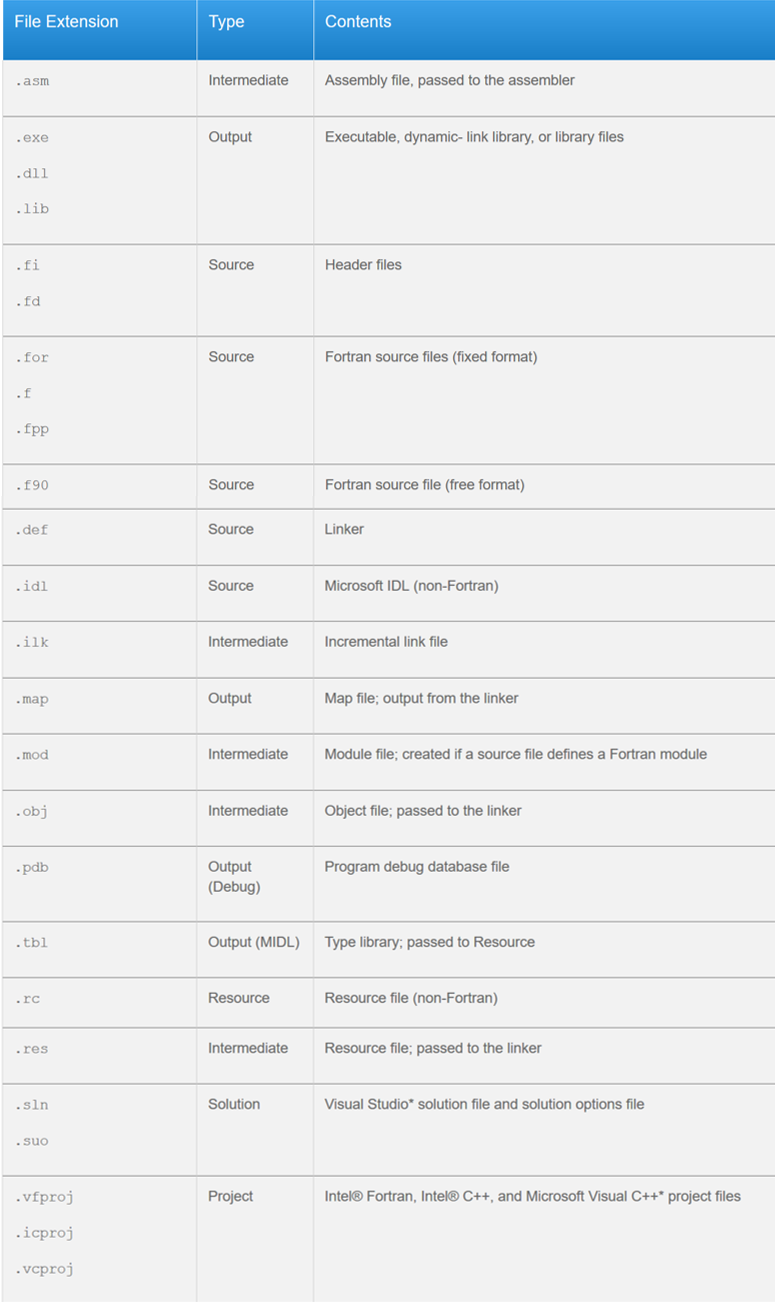
\includegraphics[width= 0.9 \textwidth]{Figures/Formats}
        \label{fig:Formats}
    \end{figure}




\end{enumerate}
